\subsection{Allgemeines}
\label{subsec:pofallgemeines}

Optische Wellenleiter, auch Lichtwellenleiter genannt, verwenden Licht zur
Übertragung von Informationen. Dies ermöglicht eine schnellere Datenübertragung
als mit Kupferkabeln. Aufgrund ihrer hohen Reichweite von mehreren Kilometern
und der hohen Übertragungsleistung von bis zu 32 Gigabit/s pro Kabel werden
Glasfaserkabel für die Verbindung von Städten und Kontinenten eingesetzt. Die
Anbindung von Gebäuden und Wohnungen an das Glasfaserkabelnetz ist mittlerweile
ein erklärtes Ziel der Telekommunikationsunternehmen. Durch Projekte wie \glqq
Fiber to the Home\grqq{} oder \glqq Fiber to the Building\grqq{} sollen
Privatpersonen und Unternehmen von hohen Übertragungsgeschwindigkeiten
profitieren. Für die Verlegung in Gebäuden sind Glasfaserkabel jedoch nur
bedingt geeignet, da Fachpersonal mit Spezialwerkzeug erforderlich ist
\cite{poflan}. Polymer optische Fasern (POF) bieten sich hier als kostengünstige
Alternative an. Sie lassen sich einfach und platzsparend verlegen (der
Durchmesser beträgt ca. 1 mm) und auf kurzen Distanzen (< 100 m) können
Datenraten von bis zu 40 Gigabit/s \cite{pofacgif} erreicht werden
\cite{pofacprofile}. POF-Kabel werden außerdem in Flugzeugen, Zügen, Automobilen
und Industrieanlagen eingesetzt. \autoref{fig:pofgrund} zeigt die Gründe für die
Verwendung in dem jeweiligen Bereich.

\begin{figure}[h]
    \begin{center}
        \begin{minipage}[t]{\textwidth}
            \begin{center}
                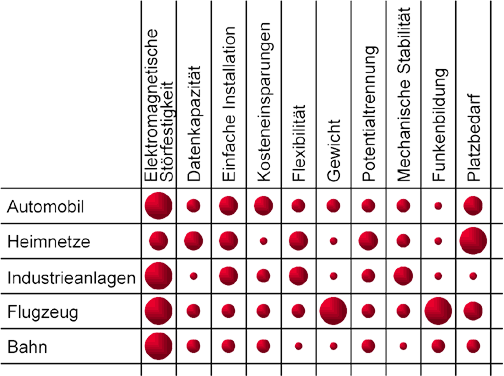
\includegraphics[height=0.2\textheight]{Bilder/Optische_Wellenleiter_Die_Polymer_Optische_Faser/Allgemeines/pofgrund.png}
                \caption[Gründe für die Verwendung von POF-Kabel \newline \url{http://www.pofac.fh-nuernberg.de/pofac/de/was_sind_pof/images/warum_pof.png} (zuletzt aufgerufen am 19.09.2015)]{Gründe für die Verwendung von POF-Kabel}
                \label{fig:pofgrund}
            \end{center}
        \end{minipage}
    \end{center}
\end{figure}

Die Größe des Kreisradius in der jeweiligen Zelle zeigt die Relevanz des
Kriteriums an.

Elektromagnetische Strahlung, elektrische Felder und Magnetfelder,
beeinträchtigen den Fluss von Elektronen in Kupferkabeln, jedoch nicht den von
Lichtstrahlen in einem Lichtwellenleiter. Daher kommen polymer optische Fasern
für die Verbindung der Sensorik zum Einsatz, da eine Störung der
Datenübertragung fatale Folgen haben könnte. Bei Flugzeugen spielen zudem
Gewicht und Funkenbildung eine große Rolle. Durch das geringe Gewicht von
POF-Kabeln reduzieren sich der Treibstoffverbrauch und damit die Betriebskosten.
Polymer optische Fasern übertragen im Gegensatz zu einem Kupferkabel keine
Elektronen sondern Licht und können somit keine Funken bilden. Damit ist eine
mögliche Gefahrenquelle eliminiert. POF-Kabel werden auch in Krankenhäusern
eingesetzt, da sie keine elektromagnetische Strahlung emittieren und deshalb
empfindliche Messgeräte nicht stören.
